\chapter{Architecture of Broadcom Cable Modems}
\label{cha:architecture}
\exploitname{} targets a vulnerable middleware running on the chip, which is used in many cable modems all over the world.
Cable modems with this chip are built with different architectures, some running a single CPU, while others run two CPUs, one for each subsystem.
As an example, the dual CPU system found in Technicolor modems can be seen in \cref{fig:overview}.
All tested cable modems are listed in \appendixref{app:ExploredRouters}, and all share the same vulnerability.

The Broadcom cable modem middleware (CM) is a real-time operating system, which runs all networking tasks, such as DOCSIS Protocol, IP-stack etc.
Along with the Broadcom middleware there usually exists a separate subsystem in the architecture, which is responsible for various things depending on the manufacture.
For instance Sagemcom uses it as a residential gateway for handling the web controller and etc. Technicolor uses it as a media server as show in \cref{fig:overview}.


\todo{update CM}
\begin{figure}[h]
  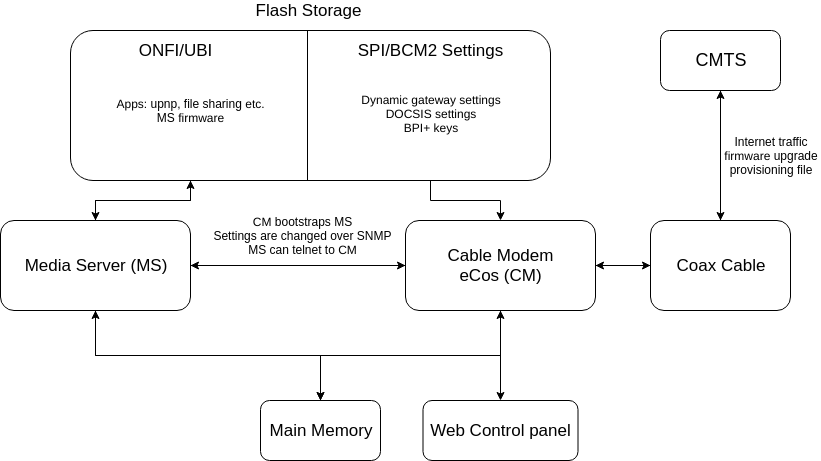
\includegraphics[width=\linewidth]{../graphics/overview.png}
  \caption{Overview of the tc7230}
  \label{fig:overview}
\end{figure}

The CM handles all of the networking protocols and the connecting to the CMTS, including firmware upgrades and keeping track of dynamic settings such as BPI+ and DOCSIS.
As all traffic goes though the CM, a would-be attacker with access to it, could listen and manipulate any traffic going through the modem.
Attempts to regain control of the modem through firmware upgrades or remote resets, can not be counted on to recover the system, as this depends on the exploited system.

\section{eCos}
\label{sec:eCos}
The CM run on a embedded multi-threaded operating system called eCos, which is widely used in embedded networking products.
This OS separate applications into tasks with fixed maximum stack size of each thread and applications can use malloc to alocate space on the heap.
Even though the stack has a fixed size threads still uses the \$sp for pushing and popping from the stack.
Applications are compiled directly into the .text part of the OS it self, meaning that the application layer is directly a part of the OS.
This also means that applications can directly manipulate OS code and data.
This OS employs few protections against potential exploits eg. no Address space layout randomization (ASLR), not protection against stack smashing, allowing stack execution etc.
This makes it easy to write exploits, as code addresses will always be at a fixed location. The OS never calls \_\_stack\_chk\_fail making it vulnerable stack buffer overflow attacks.
For these reasons finding exploits, \exploitname included, is much easier, and it is very possible that \exploitname would never be possible with a sturdier OS and architecture.